\begin{frame}
   {Raspberry-pi Zero SPI}
   \begin{figure}[H]
      \centering
      \begin{subfigure}{0.4\textwidth}
         \centering
         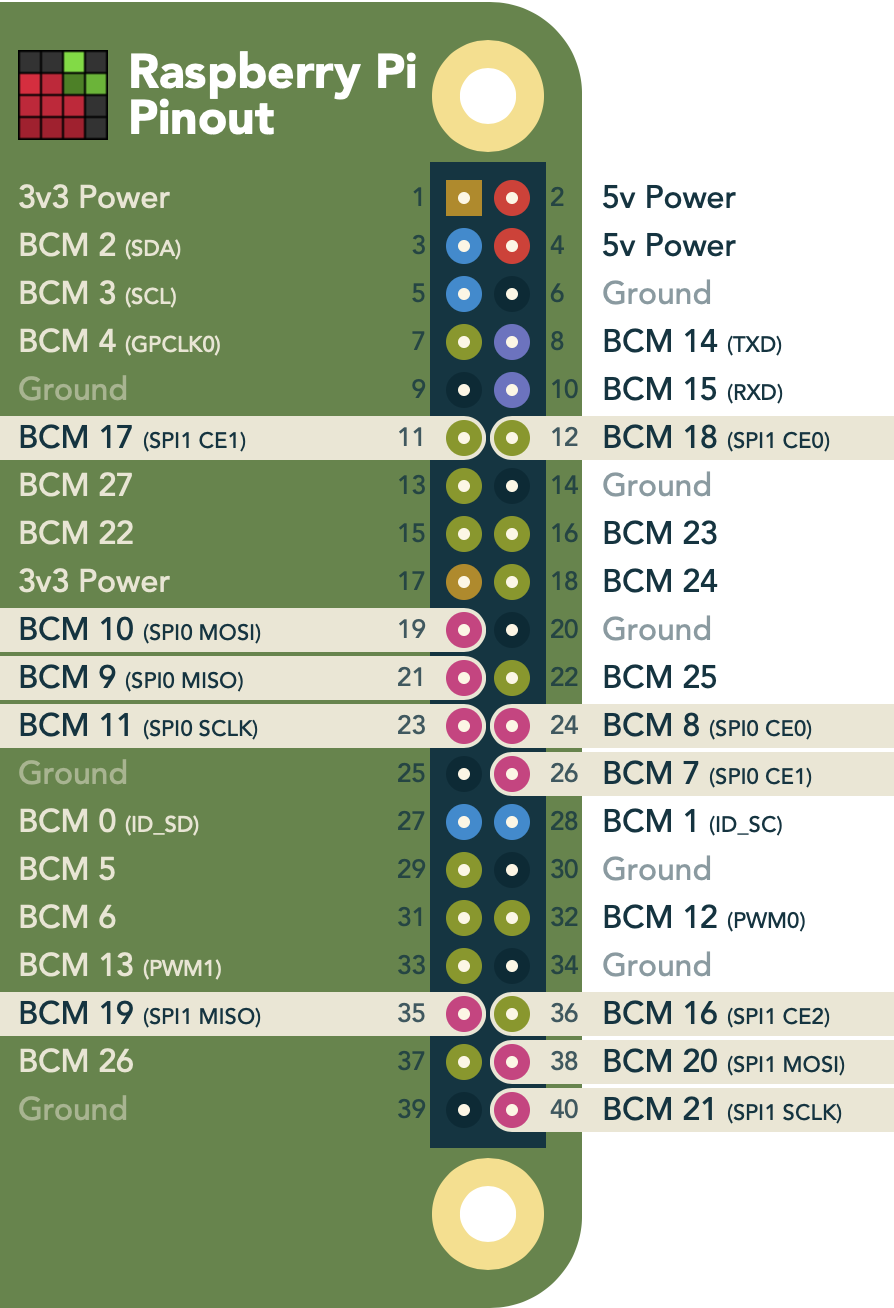
\includegraphics[height=2in]{IMAGES/rpi-pins-spi}
      \end{subfigure}
      \begin{subfigure}{0.4\textwidth}
         \centering
         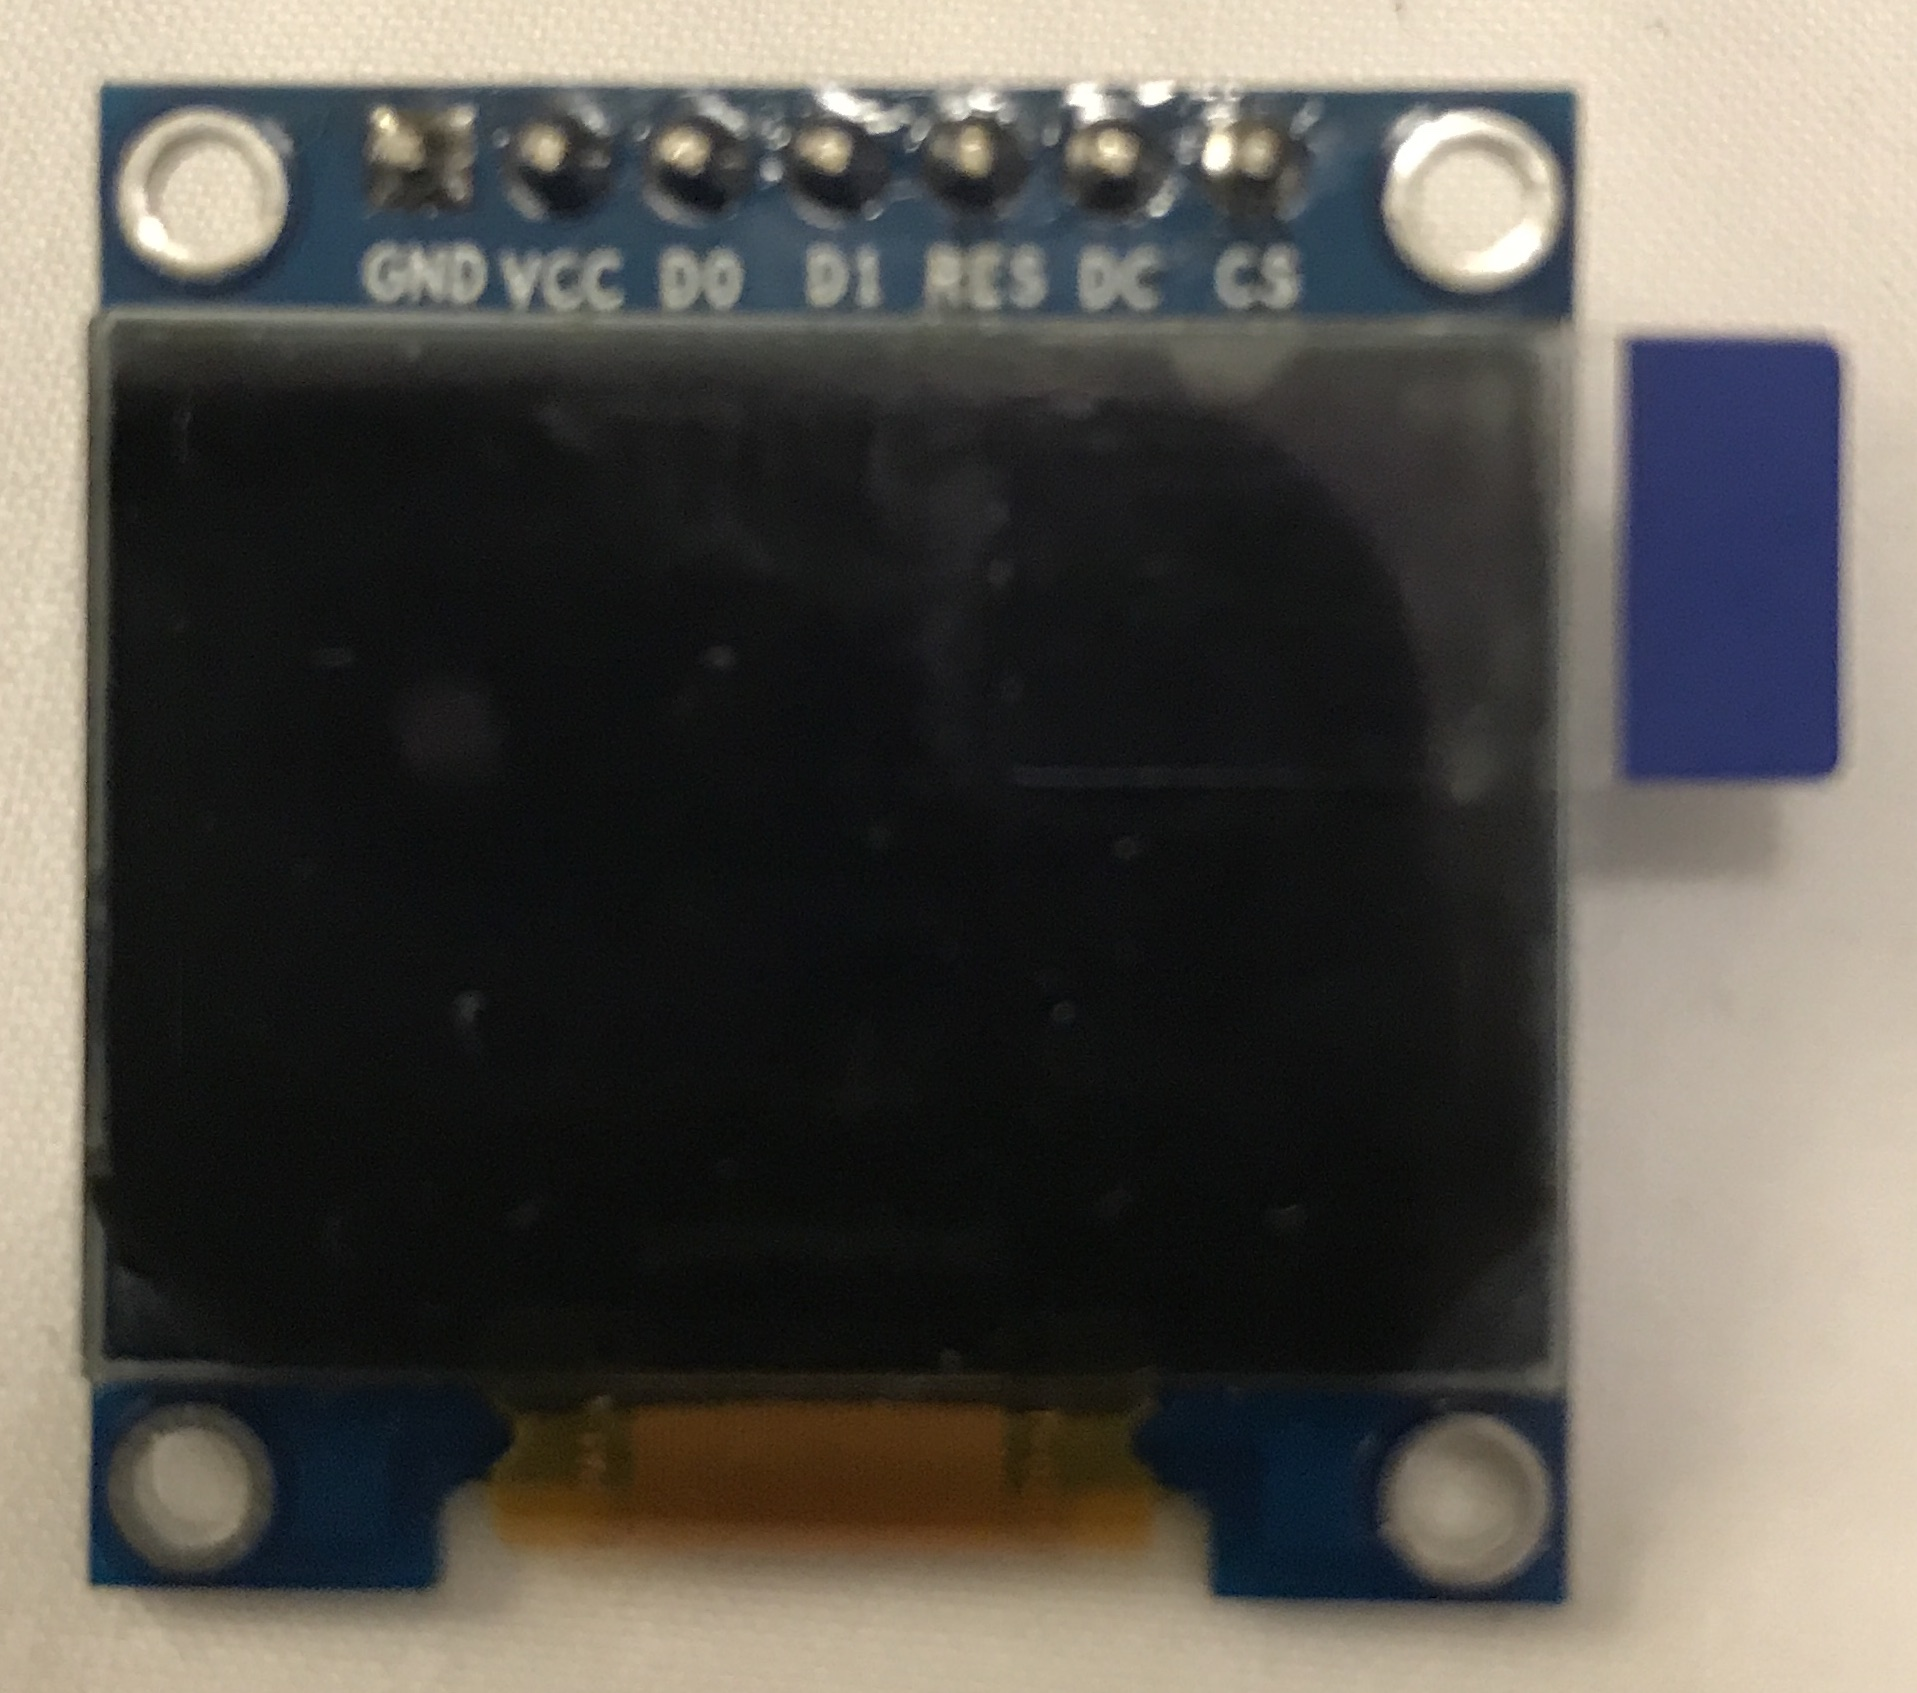
\includegraphics[height=2in]{IMAGES/SSD1306}
      \end{subfigure}
   \end{figure}
   \begin{itemize}
      \item We can access 2 SPI ports with these pins
      \item We will use one of the SPI channels to control the
	      \textbf{SSD1306 OLED screen} on the floral bonnet
   \end{itemize}
\end{frame}

\cprotect\note{

   You can learn more about the \textbf{raspberry-pi SPI pins} at pinout.xyz.

   \url{https://pinout.xyz/pinout/spi}
}

